\documentclass{article}

\usepackage{graphicx}
\usepackage{amsmath}
\usepackage[a4paper, total={14cm, 24cm}]{geometry}

\author{Mikael Henriksson \emph{and} Danyo Danev (2022)}
\title{Signal Output of a Linear Time-Variant System}
\date{}

% Typeset 'defined as'
\newcommand*{\eqdefU}{\ensuremath{\mathop{\overset{\mathrm{def}}{=}}}}

% Typeset integral from minus infinity to infinity
\newcommand*{\inft}{ \int_{-\infty}^{\infty} }

\begin{document}
\maketitle

We define the output of a Linear Time-Variant (LT) system, illustrated in Fig~\ref{fig:sys}, by the following integral equation
\begin{equation}
    y(t) \eqdefU \inft h(\tau;t) x(t-\tau) \,d\tau.
\end{equation}
Further, we define the Fourier Transform ($\mathcal{F}$) of a possibly multivariate funciton, with respect to one of its input variable, as
\begin{equation}
    \mathcal{F}_{\tau \rightarrow f} \left\{ \, h(\tau;t) \, \right\} \eqdefU \inft h(\tau;t) e^{-j2\pi f\tau} \,d\tau = H(f;t),
\end{equation}
and the Inverse Fourier Transform ($\mathcal{F}^{-1}$) of a possibly multivariate function, with respect to one of its input variables, as
\begin{equation}
    \mathcal{F}^{-1}_{f \rightarrow \tau} \left\{ \, H(f;t) \, \right\} \eqdefU \inft H(f;t) e^{j2\pi f\tau} \,df = h(\tau;t).
\end{equation}

With these three definitions, we are able to prove the following relationship between the Inverse Foruier Transform of the product
$X(f) \cdot H(f;t)$, and the time-domain output from the LT system $y(t)$:
\begin{equation}
    \begin{split}
        \inft H(f;t)X(f)e^{j2\pi ft} \, df &= \inft \inft h(w;t)e^{-j2\pi fw} \,dw \, X(f)e^{j2\pi ft} \,df = \\
        &= \inft \inft h(w;t)e^{-j2\pi fw} X(f) e^{2\pi ft} \,dw \, df = \\
        &= \inft \inft h(w;t)e^{-j2\pi fw} X(f) e^{2\pi ft} \,df \, dw = \\
        &= \inft h(w;t) \inft X(f) e^{-j2\pi fw} e^{2\pi ft} \,df \, dw = \\
        &= \inft h(w;t) \inft X(f) e^{j2\pi f(t-w)} \,df \, dw = \\
        &= \inft h(w;t) x(t-w) \, dw \eqdefU y(t).
    \end{split}
\end{equation}
We conclude the following important relation for LT systems
\begin{equation}
    \underline{\underline{y(t) \eqdefU \inft h(\tau;t) x(t-\tau) \,dx = \inft H(f;t)X(f)e^{j2\pi ft} \, df}}.
\end{equation}

\begin{figure}[]
    \centering
    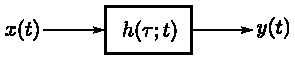
\includegraphics{lt-system.pdf}
    \caption{A general Linear and Time-Variant (LT) system.}
    \label{fig:sys}
\end{figure}

\end{document}
